% Chapter 4b
\chapter{Object Reconstruction in the ATLAS Detector} % Chapter title
\label{ch:reconstruction} 

Object reconstruction is the computation-intensive process of turning the signals from the approximately 100 million read-out channels of the ATLAS detector into a collection of particles and jets, the objects with which physics analysis can be performed. This process is complicated, and requires dedicated working groups in the ATLAS experiment that optimize the understanding of each type of object, which must all collaborate to provide a full picture of the events in the detector.

%---------------------------------------------------------------------------------------

\section{Electrons}
\label{sec:reco_electrons}

Electrons are identified through a combination of \ac{ID} and calorimeter measurements. They travel through the tracking system, leaving charge deposits in each layer, then are absorbed by the electromagnetic calorimeter. These two measurements work in conjunction to deliver high resolution measurements of electron momentum from low-\pt, where track curvature gives the most reliable measure of the electron's energy, to high-\pt, where the tracks are almost perfectly straight, but the calorimeter can still provide a reliable measurement. 

In the central region ($|\eta|<2.47$) of the ATLAS detector, electron reconstruction begins with the identification of energy deposits in the electromagnetic calorimeter. The calorimeter clusters are seeded by sliding longitudinal windows, which are measured in units of 0.025 in $\eta$ and $\phi$. 3$\times$5 unit windows are used, which require at least 2.5 \gev~in the window to form a seed \cite{Aad:2011mk}. 

These clusters are matched to \ac{ID} tracks by extrapolating the track to the middle layer of the calorimeter and identifying nearby clusters. If there are multiple tracks associated with a given cluster, tracks with silicon hits are preferentially chosen, and then the track with the smallest $\Delta R$ to the center of the cluster is selected. The track is used to determine the likely direction of bremsstrahlung radiation in the calorimeter, and the seed cluster window is expanded in $\phi$ to included the radiation. 

The calorimeter clusters are then rebuilt in in larger windows, 3$\times$7 in the barrel and 5$\times$5 in the end-caps. An estimate of the energy is made by summing the measured calorimeter energy with estimates of the energy lost before the electron reached the calorimeter, energy outside of the cluster window, and energy not fully deposited in the calorimeter. These estimates are made with parametrized functions determined from a comparison of \ac{MC} and measurements taken by the presampler. 

The momentum is determined though a combination of the calorimeter and track measurements of the electron, while its $\eta$ and $\phi$ are taken from the track at its vertex. The energy of the electron is taken from the calorimeter cluster.

In the forward region, where no tracking is available, electron energy is determined more roughly. Calorimeter cells are formed into variable-sized clusters in regions of significant energy deposition, and the center of the cluster is used to determine angular coordinates of the electron. 

Electrons are identified using an algorithm that uses multivariate analysis to assign a likelihood that a candidate is a true electron based on input from just under twenty different variables. These include track quality, hadronic leakage, and cluster shape, incorporating information from as many subdetectors as possible in its determination of the candidate's quality. Each variable is assigned a \ac{PDF} for true electrons and background processes, and they are collectively used to provide a likelihood value which can be cut on. 

Three levels of identification, \texttt{LHLoose}, \texttt{LHMedium}, and \texttt{LHTight}, are defined with different likelihood cuts, with tighter cuts always a subset of the looser cuts. \autoref{fig:reco_el_eff} gives the efficiencies at each of these working points both for true electrons and for hadrons, which can be misidentified as electrons. Tighter working points have worse efficiencies, but lower misidentification rates. 

\begin{centering}
\begin{figure}[!hbt]
\myfloatalign
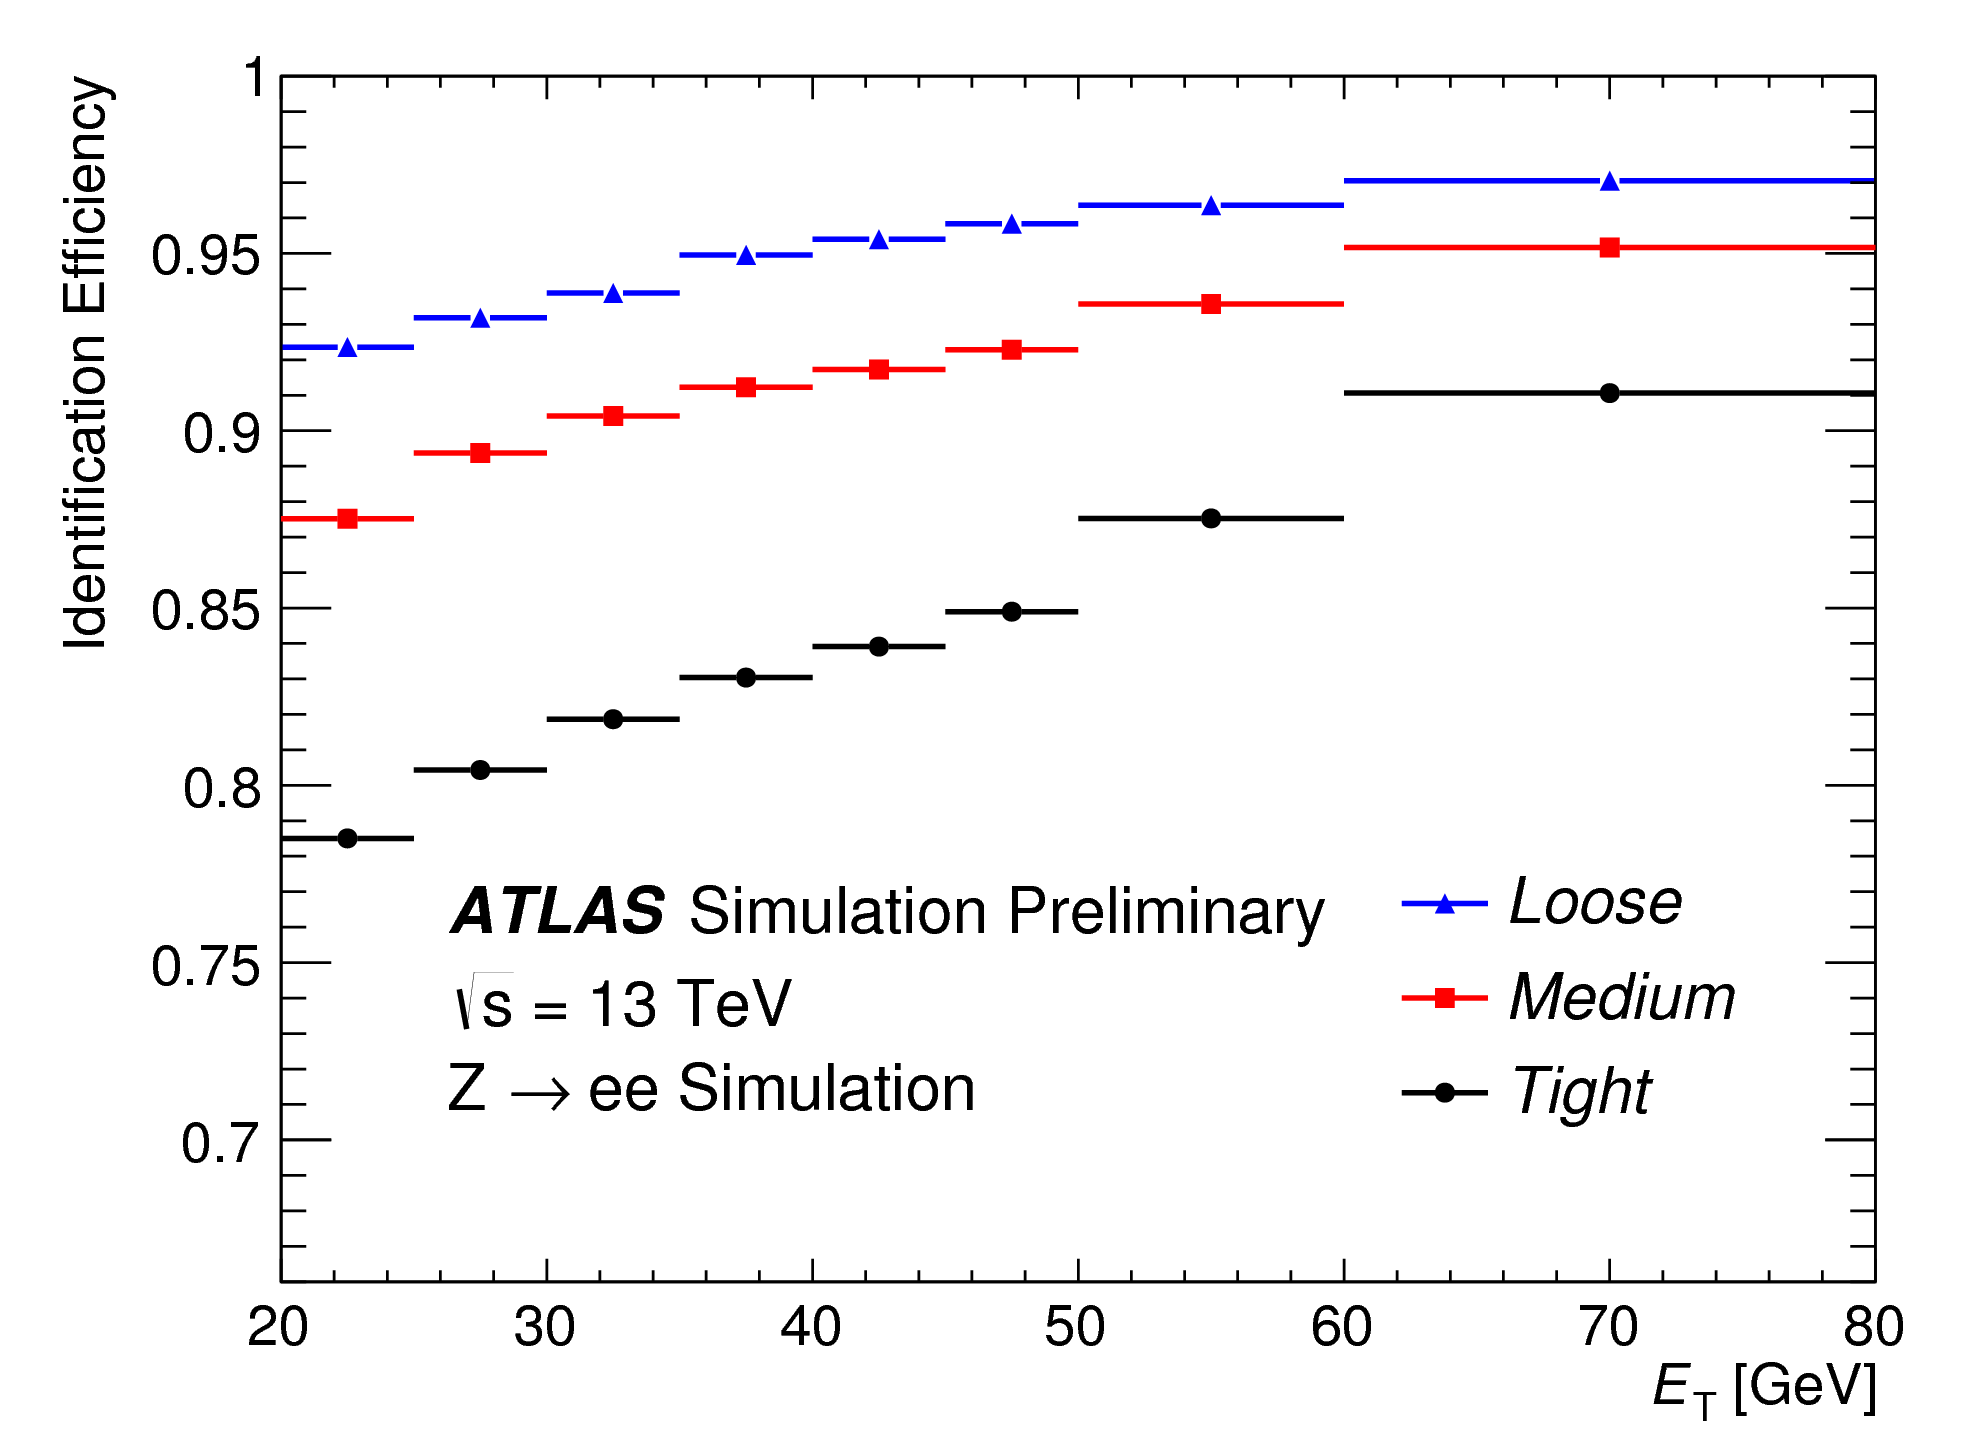
\includegraphics[width=.48\linewidth]{figures/reco/fig_01a.png}
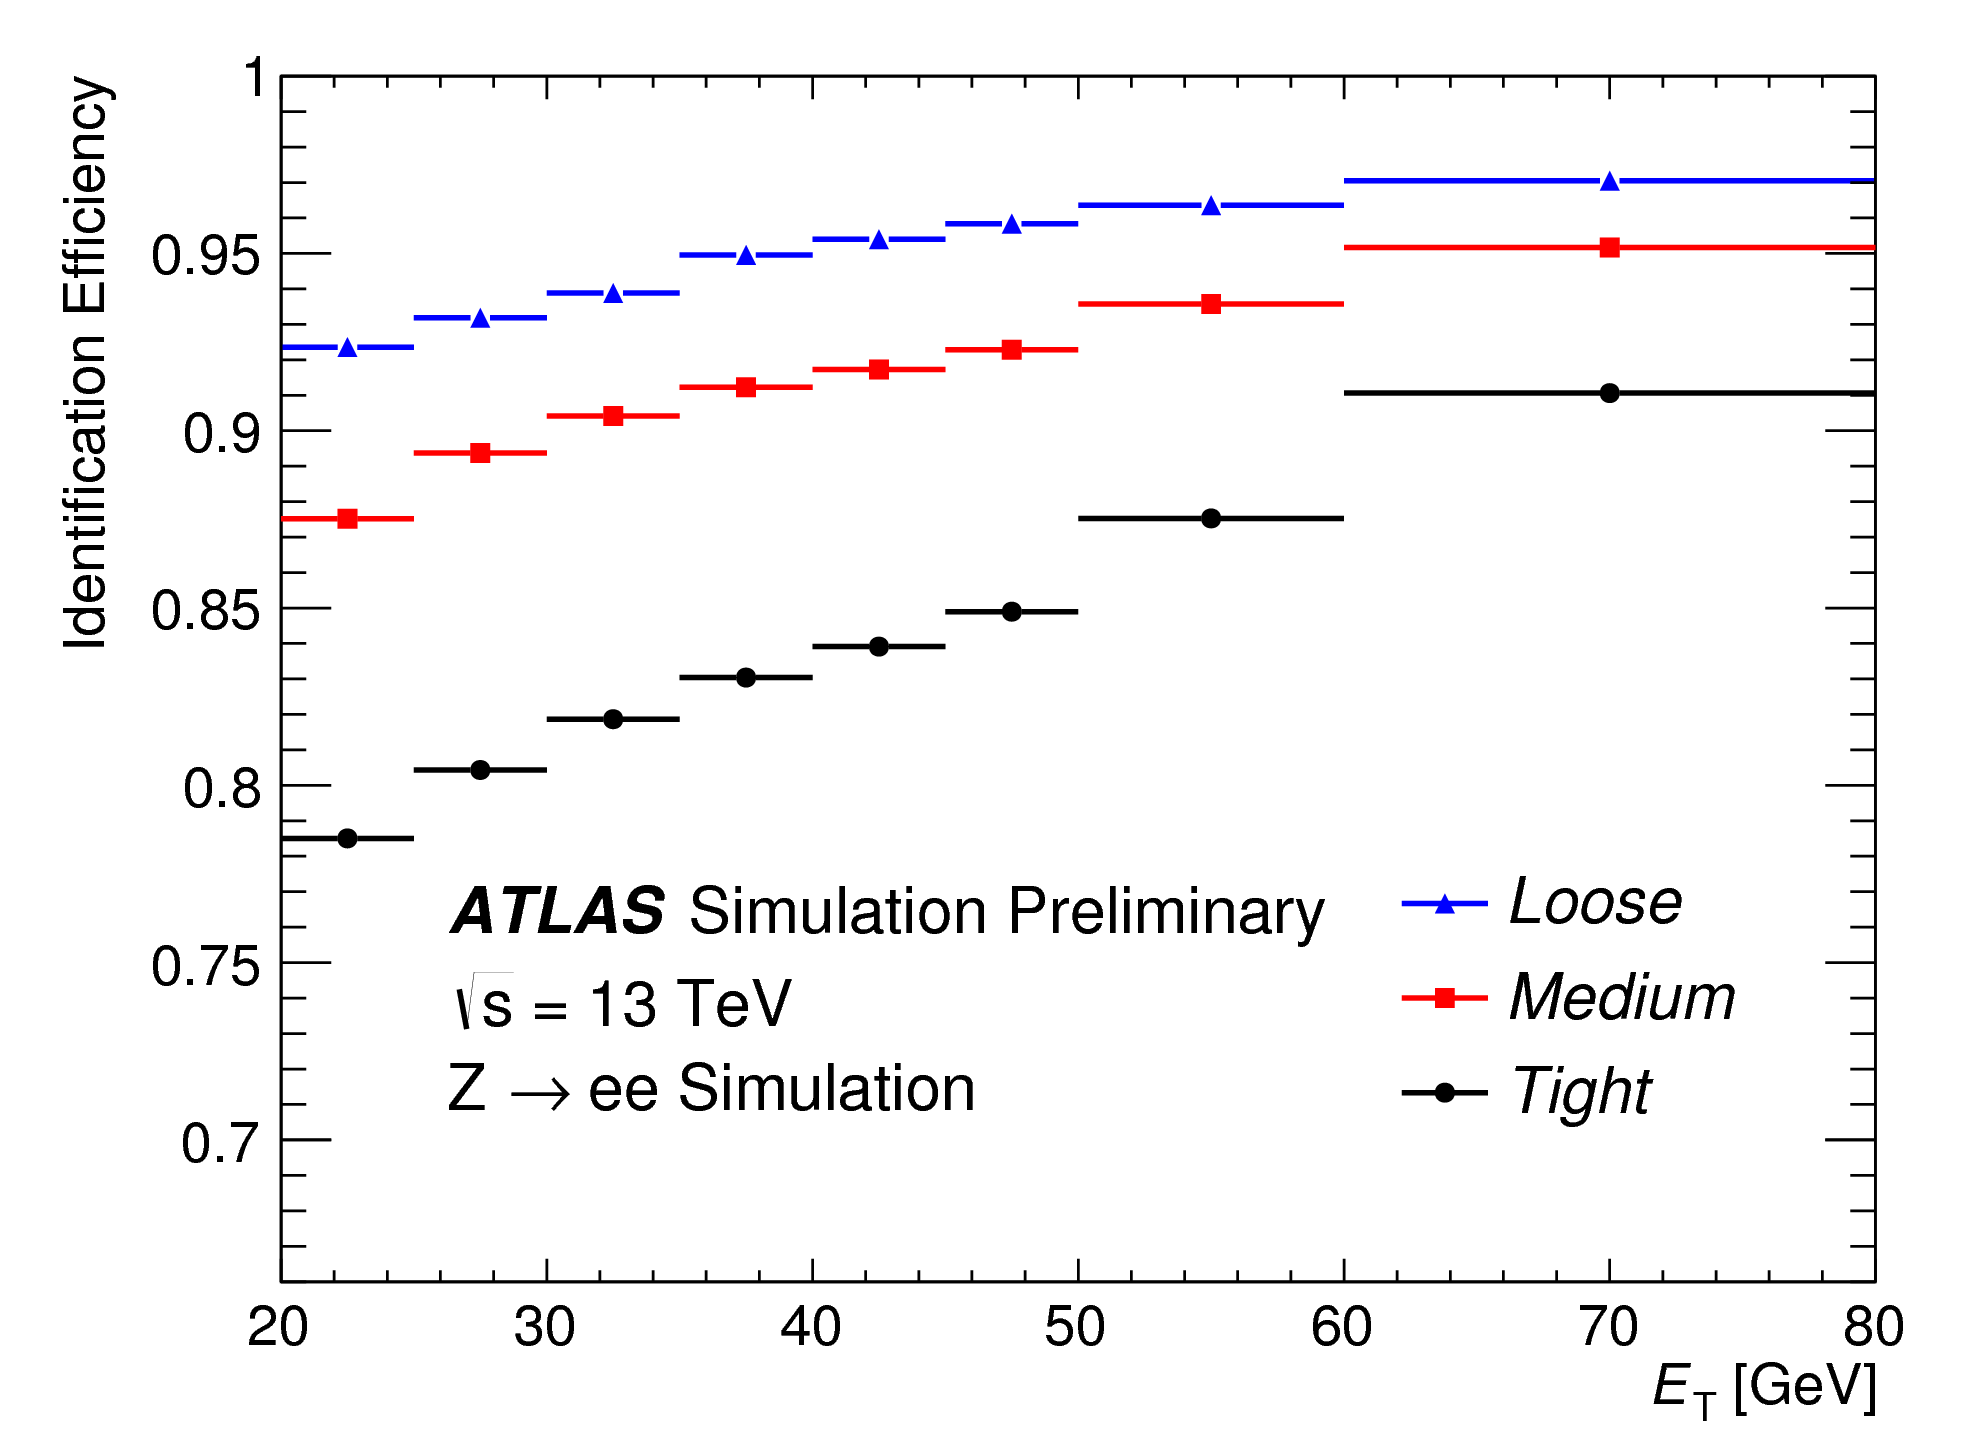
\includegraphics[width=.48\linewidth]{figures/reco/fig_01a.png}
\caption{ Identification efficiencies from \ac{MC} samples for loose, medium, and tight working points. Left is the efficiency for identification of true electrons taken from $Z\rightarrow ee$ \ac{MC}, and right is the efficiency for mis-identification of jets as electrons taken from dijet \ac{MC} \cite{ATLAS-CONF-2016-024}.}
\label{fig:reco_el_eff}
\end{figure}
\end{centering}

\ac{MC} efficiencies can be compared to efficiencies measured in data using the tag-and-probe method, to obtain a \textit{scalefactor}, a correction factor applied to \ac{MC} to better emulate the rates at which electrons are reconstructed and identified. \autoref{fig:reco_el_sf} shows a comparison of the combined reconstruction and identification efficiencies in data and \ac{MC}, with the resulting scalefactors also displayed as the ratio. 

\begin{centering}
\begin{figure}[!hbt]
\myfloatalign
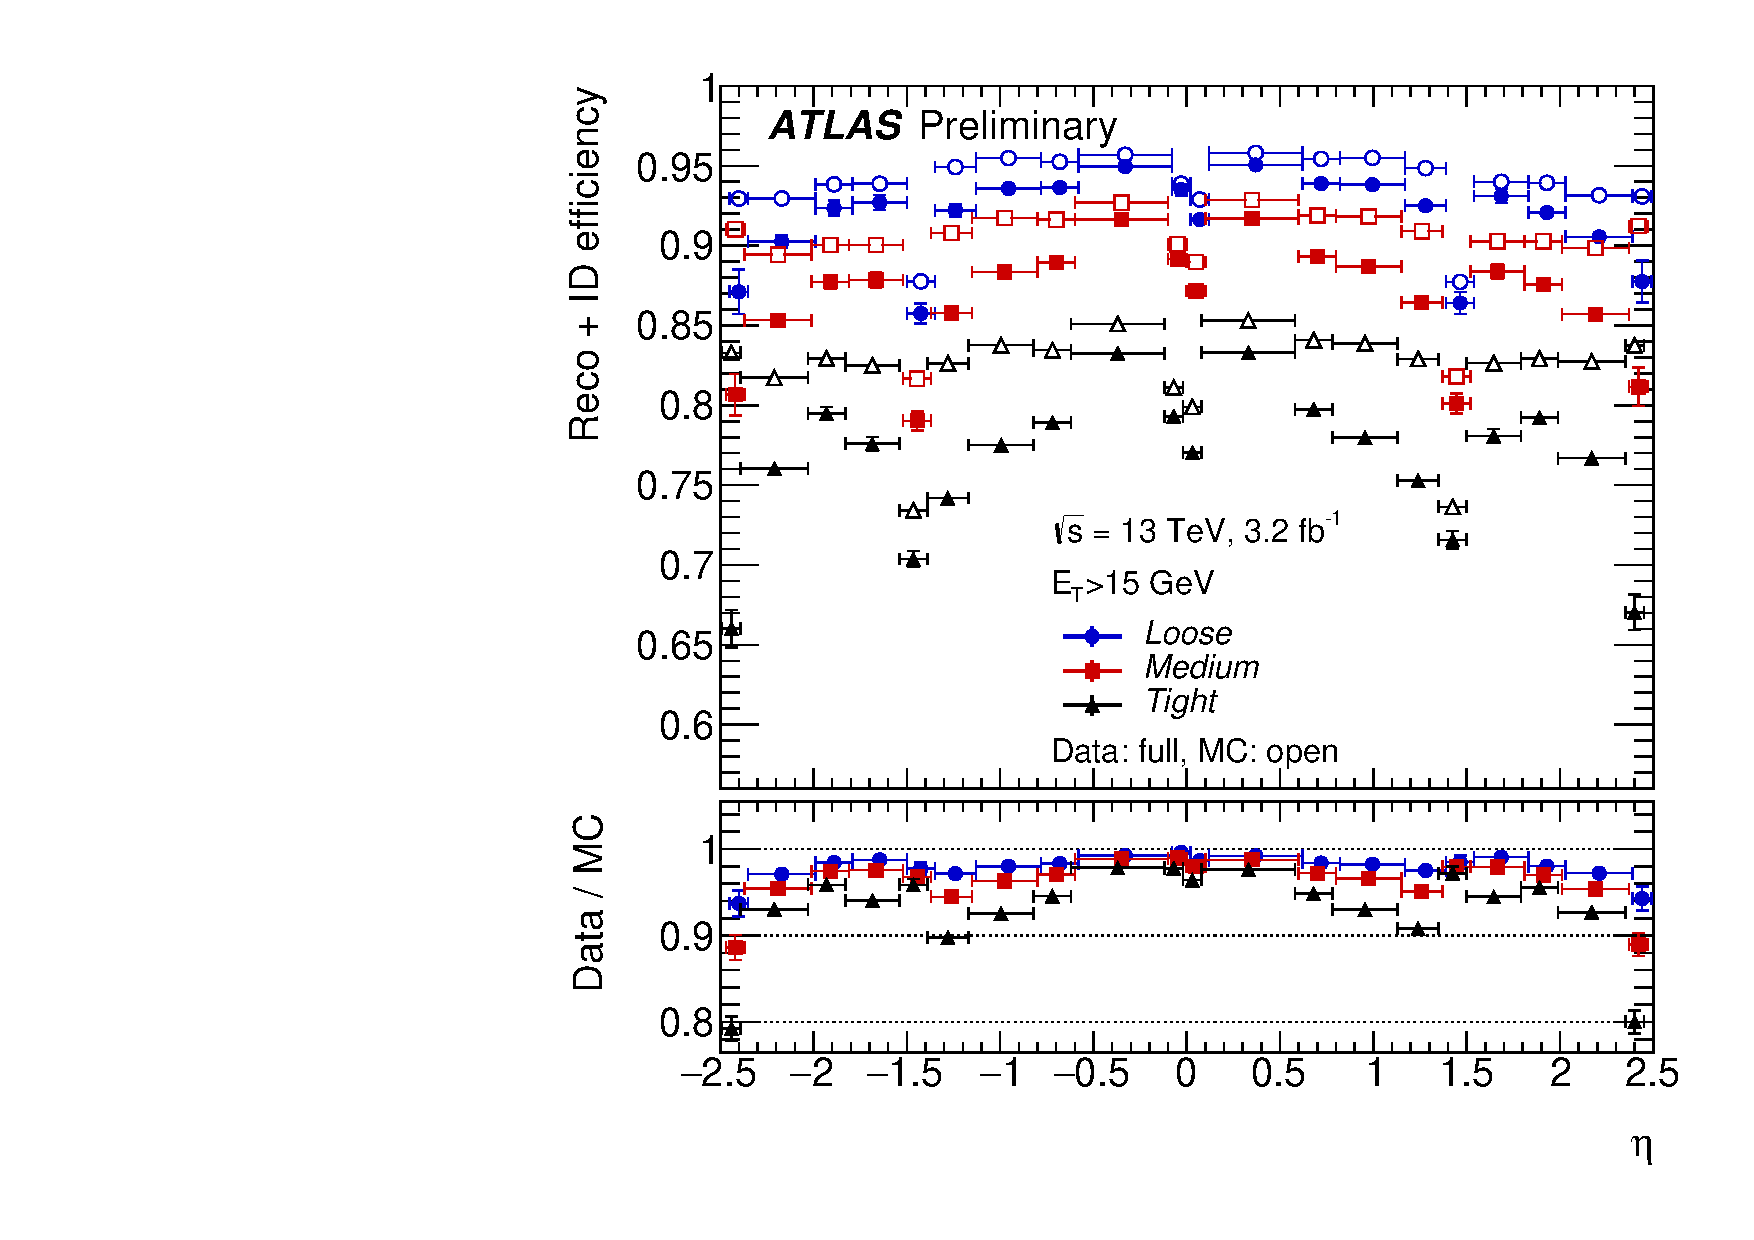
\includegraphics[width=.90\linewidth]{figures/reco/fig_14b.pdf}
\caption{ Combined electron reconstruction and identification efficiencies measured as a function of $\eta$ for data (using the tag-and-probe method on $Z\rightarrow ee$ events) and $Z\rightarrow ee$ \ac{MC}. Distributions include all electrons with \et > 15 \gev. \cite{ATLAS-CONF-2016-024}.}
\label{fig:reco_el_sf}
\end{figure}
\end{centering}

Electrons can also have \textit{isolation} requirements, cuts on nearby calorimeter activity or tracks. Isolation variables are primarily used to reject non-prompt leptons, which can be produced in heavy flavor hadron decays, converted photons, and misidentified hadrons. Cuts are made on the amount of nearby calorimetric energy and sum of the \pt of nearby tracks relative to the electron's energy, forming a series of working points. Fixed cut working points, which specify the relative fraction to cut on, can be used, but efficiency targeted working points are more popular. These include \texttt{Tight} and \texttt{Loose} working points, which operate at 95 and 98\% efficiency respectively, and working points that target tighter efficiencies at higher electron \pt, \texttt{Gradient} and \texttt{GradientLoose}. These working points each have 99\% efficiency for electrons with \pt > 60 \gev, but 90 and 95\% efficiencies at 25 \gev. 

\section{Photons}
\label{sec:reco_photons}



\section{Muons}
\label{sec:reco_muons}



\section{Jets}
\label{sec:reco_jets}


\section{Overlap Removal}
\label{sec:reco_or}



\section{Missing Transverse Energy}
\label{sec:reco_met}

Another common usage is $E_T^{miss}$, which gives the negative vectorial sum of the energy in an event. 



